\newpage % Rozdziały zaczynamy od nowej strony.
 

\section{Użyte metody}
W tym rozdziale opiszę użyte przez siebie metody prowadzące, od zbioru kodów źródłowych programów, do działającej wtyczki 
przewidującej kolejny token w programie. Omówię również hipotezy zerowe oraz alternatywne dla pytań postawionych w wstępnym rozdziale.\\\\\\ 

\subsection{Badane modele}
Rekurencyjne sieci neuronowe należą do rodziny sieci służących do przetwarzania sekwencji danych o określonej długości. Jak pokazali w swojej publikacji 
Shewalkar, Nyavanandi i Ludwig \cite{lstmvsgru}, sieć LSTM osiąga znacznie lepsze wyniki od podstawowej sieci rekurencyjnej RNN oraz minimalnie lepsze wyniki 
od sieci GRU, kosztem dłuższego czasu treningu. Z tego względu w swoich badaniach skupiam się głównie na warstwie LSTM oraz w mniejszej mierze na warstwie GRU, 
która również wyprzedza podstawową sieć RNN pod względem skuteczności. 

Wszystkie eksperymenty badające wpływ hiperparametrów wymienionych w wstępnym rozdziale \ref{questions} przeprowadzę na sieci LSTM, oraz najlepszą ich kombinację 
zbadam przy wykorzystaniu warstwy GRU w celu porównania ich skuteczności w zadaniu przewidywaniu kodu. Na koniec zbadam również zachowanie wyznaczonego modelu 
dla różnych rozmiarów słownika. 

Jak pokazał w swojej pracy Yoon Kim \cite{kim} połączenie warstwy rekurencyjnej z warstwą zanurzeń poprzez warstwę splotową może mieć pozytywny wpływ na skuteczność 
modelu. Jednak badanie to wykonywał jedynie w zadaniu modelowania języka naturalnego oraz dla modeli opartych na pojedyńczych znakach. Jednym z wykonanych przeze mnie 
eksperymentów będzie zastosowanie tej techniki w moim zadaniu, oraz oceny skuteczności tego podejścia dla modeli opartych na tokenach. \\\\\\

\begin{figure}[!h]
	% Znacznik \caption oprócz podpisu służy również do wygenerowania numeru obrazka;
	\caption{Ogólny badany model. Opcjonalne warstwy zaznaczone linią przerywaną}
	% dlatego zawsze pamiętaj używać najpierw \caption, a potem \label
    \label{fig:architektura}
    % Zamiast width można też użyć height, etc. 
    \centering 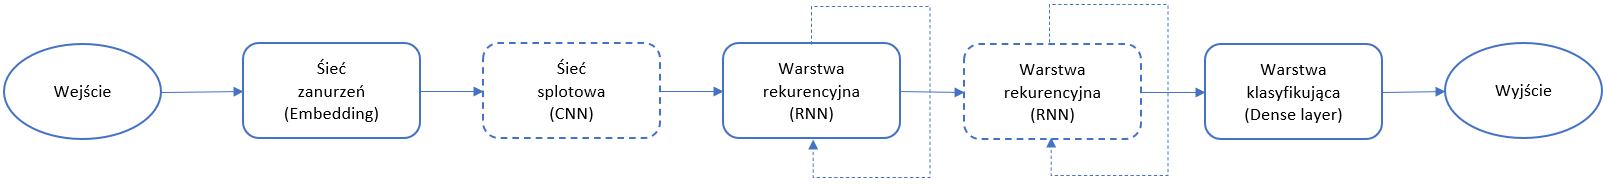
\includegraphics[width=160mm, height=25mm]{architektura.png}
\end{figure}


\begin{table}[ht]
    \centering
    \resizebox{\textwidth}{!}{\begin{tabular}{ccccc}
            \hline
            \multicolumn{1}{|c|}{Długość sekwencji}   & \multicolumn{1}{c|}{Warstwa CNN}          & \multicolumn{1}{c|}{Liczba warstw LSTM} & \multicolumn{1}{c|}{Liczba neuronów w warstwie} & \multicolumn{1}{c|}{Liczba wszystkich parametrów} \\ \hline
            \multicolumn{1}{|c|}{1}                   & \multicolumn{1}{c|}{nie}                  & \multicolumn{1}{c|}{1}                  & \multicolumn{1}{c|}{512}                        & \multicolumn{1}{c|}{todo}                         \\ \hline
            \multicolumn{1}{|c|}{\multirow{5}{*}{5}}  & \multicolumn{1}{c|}{\multirow{4}{*}{nie}} & \multicolumn{1}{c|}{\multirow{3}{*}{1}} & \multicolumn{1}{c|}{128}                        & \multicolumn{1}{c|}{todo}                         \\ \cline{4-5} 
            \multicolumn{1}{|c|}{}                    & \multicolumn{1}{c|}{}                     & \multicolumn{1}{c|}{}                   & \multicolumn{1}{c|}{256}                        & \multicolumn{1}{c|}{todo}                         \\ \cline{4-5} 
            \multicolumn{1}{|c|}{}                    & \multicolumn{1}{c|}{}                     & \multicolumn{1}{c|}{}                   & \multicolumn{1}{c|}{512}                        & \multicolumn{1}{c|}{todo}                         \\ \cline{3-5} 
            \multicolumn{1}{|c|}{}                    & \multicolumn{1}{c|}{}                     & \multicolumn{1}{c|}{2}                  & \multicolumn{1}{c|}{128}                        & \multicolumn{1}{c|}{todo}                         \\ \cline{2-5} 
            \multicolumn{1}{|c|}{}                    & \multicolumn{1}{c|}{tak}                  & \multicolumn{1}{c|}{1}                  & \multicolumn{1}{c|}{128}                        & \multicolumn{1}{c|}{todo}                         \\ \hline
            \multicolumn{1}{|c|}{\multirow{5}{*}{10}} & \multicolumn{1}{c|}{\multirow{4}{*}{nie}} & \multicolumn{1}{c|}{\multirow{2}{*}{1}} & \multicolumn{1}{c|}{128}                        & \multicolumn{1}{c|}{todo}                         \\ \cline{4-5} 
            \multicolumn{1}{|c|}{}                    & \multicolumn{1}{c|}{}                     & \multicolumn{1}{c|}{}                   & \multicolumn{1}{c|}{512}                        & \multicolumn{1}{c|}{todo}                         \\ \cline{3-5} 
            \multicolumn{1}{|c|}{}                    & \multicolumn{1}{c|}{}                     & \multicolumn{1}{c|}{2}                  & \multicolumn{1}{c|}{128}                        & \multicolumn{1}{c|}{todo}                         \\ \cline{3-5} 
            \multicolumn{1}{|c|}{}                    & \multicolumn{1}{c|}{}                     & \multicolumn{1}{c|}{2}                  & \multicolumn{1}{c|}{512}                        & \multicolumn{1}{c|}{todo}                         \\ \cline{2-5} 
            \multicolumn{1}{|c|}{}                    & \multicolumn{1}{c|}{tak}                  & \multicolumn{1}{c|}{1}                  & \multicolumn{1}{c|}{126}                        & \multicolumn{1}{c|}{todo}                         \\ \hline
            \multicolumn{1}{|c|}{\multirow{2}{*}{15}} & \multicolumn{1}{c|}{\multirow{2}{*}{nie}} & \multicolumn{1}{c|}{\multirow{2}{*}{1}} & \multicolumn{1}{c|}{128}                        & \multicolumn{1}{c|}{todo}                         \\ \cline{4-5} 
            \multicolumn{1}{|c|}{}                    & \multicolumn{1}{c|}{}                     & \multicolumn{1}{c|}{}                   & \multicolumn{1}{c|}{512}                        & \multicolumn{1}{c|}{todo}                         \\ \hline
                                                      &                                           &                                         &                                                 &                                                  
            \end{tabular}}
    \caption{Zestawienie wykonywanych eksperymentów} 
    \end{table} 

\subsection{Hipotezy}
todo
    
\subsection{Modelowanie tokenów}
Jak pokazuje w swojej publikacji Hao Peng wraz z zespołem \cite{character-level} mimo tego, że modele budujące kolejne słowa poprzez 
przewidywanie pojedyńczego znaku (character-level model) radzą sobie dobrze z modelowaniem języka naturalnego oraz rozwiązują problem rozmiaru słownika, 
działają znacznie gorzej z językami programowania. Wniosek ten również potwierdza w swojej pracy Erik van Scharrenburg \cite{erik} porównując model przewidujący 
znaki z modelem przewidującym tokeny. Z tego powodu w  realizuję tylko modele oparte na tokenach (token-level model). 

Pierwszym krokiem jest zbudowania słownika tokenów, które mogą pojawić się w kodzie. Buduję go poprzez przetworzenie wszystkich kodów źródłowych obu zbiorów treningowego oraz 
walidacyjnego modułem tokenize \cite{tokenize} wbudowanym w język Python. Moduł ten przyjmuje na wejściu kod źródłowy programu następnie zwraca listę kolejnych tokenów (nazw zmiennych, 
znaków specjalnych, słów kluczowych). Upewnia się on również czy kod jest poprawnie napisany np. czy wszystkie nawiasy lub apostrofy zostały zamknięte. Niepoprawne programy pomijam. 
Znaki nowej lini również traktuję jako token, jednak nie uwzględniam wcięć w kodzie ze względu na to, że większość środowisk programistycznych stawia je 
automatycznie. Na przykład z kodu źródłowego: 
\begin{addmargin}[10mm]{0mm}
    \begin{lstlisting}[
        language=Python,
        numbers=left,
        firstnumber=1,
        caption={Przykładowy program Python},
        aboveskip=10pt
    ]
    for x in range(2, 10): 
        print("hello world")
    \end{lstlisting}
    \end{addmargin}
otrzymamy listę \textbf{ [for, x, in, range, (, 2, 10, ), :, \textbackslash n, print, (, "hello world", )] }.
Następnie sortuje wszystkie wygenerowane tokeny według częstości występowania oraz wybieram top-n tokenów jako słownik i każdemu z nich przypisuję unikalną liczbę naturalną. 
Utworzony w ten sposób słownik nie jest kompletny ponieważ nie obejmuje on wszystkich możliwych nazw występujących w kodzie. Takiego rodzaju tokeny
zostają zastąpione sztucznym tokenem '<UNKNOWN>'. W głównej mierze są to unikalne nazwy zmiennych oraz stringi. Zastępowanie tokenu '<UNKNOWN>' prawdziwym prawdziwym tokenem omówię w 
poświęconym temu rozdziale. 

\subsection{Wybór podzbioru danych}
Jak już wspomniałem w sekcji \ref{sec:dataset-background} dotyczącej zbioru danych, trening odbywa sie na podzbiorze wszystkich zgromadzonych danych. W tym celu wybrałem 9 najpopularniejszych 
zewnętrznych bibliotek języka Python stosowanych do zróżnicowanych dziedzin rozwoju oprogramowania. Poniżej zamieszam listę wybranych bibliotek wraz z krótkim opisem:
\begin{itemize}
    \item Django - rozwój aplikacji sieciowych
    \item Numpy - wykonywanie obliczeń matematycznych wysokiego poziomu
    \item Requests - wysyłanie zapytań http 
    \item Flask - rozwój aplikacji sieciowych  
    \item TensorFlow - Głębokie uczenie maszynowe
    \item Keras - Wysokopoziomowe uczenie maszynowe
    \item PyTorch - Głębokie uczenie maszynowe
    \item Pandas - Zarządzanie dużymi zbiorami danych
    \item PyQt - Tworzenie interfejsów użytkownika
\end{itemize} 
Aby upewnić się, że wybrany przeze mnie zbiór danych poprawnie oddaje rzeczywistość porównałem liczbę plików źródłowych zwierających konkretną bibliotekę ze zbioru z odpowiadającą 
liczbą plików źródłowych na platformie GitHub \cite{github}. 
\begin{table}[!h] \centering
    % Znacznik \caption oprócz podpisu służy również do wygenerowania numeru tabeli;
    \caption{Zestawienie zbioru danych z platformą GitHub}
    % dlatego zawsze pamiętaj używać najpierw \caption, a potem \label.
    \label{tab:dataset-compare}
    
    \begin{tabular} {| c | c | r | r |} \hline
        Biblioteka & Liczba plików GitHub & Liczba plików w zbiorze danych & stosunek\\\hline\hline
        Django & 187000000 & 26732 & 0.014\% \\\hline
        Numpy & 55000000 & 9058 & 0.016\% \\ \hline
        Requests & 42000000 & 6339 & 0.015\%\\ \hline
        Pandas & 19000000 & 1328 & 0.007\%\\ \hline
        Flask & 17000000 & 3230 & 0.019\% \\ \hline
        TensorFlow & 10000000 & 96 & 0.001\%\\ \hline
        Keras & 3000000& 72 & 0.002\%\\ \hline
        PyQt & 1000000 & 132 & 0.013\%\\ \hline
        PyTorch & 1000000 & 0 & 0\%\\ \hline
    \end{tabular}
\end{table}

Jak możemy zaobserwować stosunek liczby plików jest dosyć zbliżony dla większości wybranych bibliotek wynosi około 0.015\%, z wyjątkiem 
bibliotek uczenia maszynowego. Może to wynikać z tego, że dane pochodzą z 2018 roku oraz jest to czas, w którym istniały początkowe wersje tych bibliotek oraz dopiero
zaczynały zyskiwać na popularności. Od tego czasu również biblioteka Keras została scalona z biblioteką TensorFlow co znacznie wpłynęło na jej popularność w dzisiejszych czasach. 

Uznaję, że dane w wystarczająco dobrym stopniu oddają częstotliwość zastosowania bibliotek. Końcowy podzbiór stworzyłem poprzez wybranie 1\% plików źródłowych z każdej biblioteki. 
Końcowe zestawienie prezentuje się w następujący sposób:

\begin{table}[!h] \centering
    % Znacznik \caption oprócz podpisu służy również do wygenerowania numeru tabeli;
    \caption{Zestawienie zbioru i podzbioru danych}
    % dlatego zawsze pamiętaj używać najpierw \caption, a potem \label.
    \label{tab:dataset-compare-github}
    
    \begin{tabular} {| c | c | r | r |} \hline
         & Cały zbiór danych & Podzbiór treningowy & Podzbiór walidacyjny \\\hline\hline
        Pliki & 150000 & 9103 & 4504 \\\hline
        Tokeny & 114641650 & 9118453 & 4482600 \\ \hline
    \end{tabular}
\end{table}
Rozmiar wykorzystanego zbioru danych jest podobny do zbioru użytego w publikacjach Vincent J. Hellendoorn i Premkumar Devanbu \cite{hellendoorn} w którym użyto 16 milionów tokenów do treningu, oraz 
5 milionów tokenów w celach walidacji. Na różnicę tą zdecydowałem się ze względu na ograniczenia sprzętowe różniące oba projekty. 


\subsection{Trening}
Zadanie polega na przewidzeniu kolejnego tokenu na podstawie zadanej sekwencji tokenów. Długość sekwencji jest stała oraz wyrażona poprzez wielkość okna będącą jednym z badanych hiperparametrów. 
Dla każdego z tokenów model wyszukuje jego wektor zanurzenia, wykonuje jeden krok w sieci rekurencyjnej po czym stosuje warstwę klasyfikującą 
(Dense layer) w celu wygenerowania logitów wyrażających logistyczne-prawdopodobieństwo kolejnego tokenu. Zatem dla zadanego okna tokenów długości \begin{math}W\end{math}:
\begin{math}[t_1, t_2, ... t_W]\end{math} obliczam wynik dla każdego możliwego wyjścia \begin{math}j, s_j\end{math} jako funkcję z wektorów tokenów \begin{math}v_{t_i}\end{math}
z tokenów z okna.
\\
\centerline{\begin{math}[g_1, g_2, ..., g_W] = RNN([v_{t_1}, v_{t_2}, ..., v_{t_W}])\end{math}}\\
\centerline{\begin{math}s_j=p_{j}^{T}[g]\end{math}} \\\\
Minimalizowana funkcja strat jest entropią krzyżową pomiędzy prawdopodobieństwami \begin{math}softmax\end{math} dla każdego możliwego wyjścia 
a wykonaną predykcją.Funkcja wyrażoną wzorem: \\\\
\centerline{\begin{math}L = log(\frac{e^{s_{t_o}}}{\sum_{j}e^{s_{t_j}}})\end{math}}\\\\
gdzie \begin{math}t_o\end{math} jest zaobserwowanym tokenem wyjściowym a \begin{math}g_i\end{math} wyjściem \begin{math}i^{th}\end{math} komórki
którejś z badanych sieci rekurencyjnych. 

Wagi sieci aktualizowane są po przetworzeniu porcji danych (mini-batch) której rozmiar jest stały. Przy treningach sieci rekurencyjnych rozmiar
ten jest jedną z wartości kluczowych dla dobrej wydajności sieci. W moich eksperymentach wynosi on 128. Jest to kompromis pomiędzy rozsądnym 
czasem treningu oraz jakością wyjściowych sugestii. Jest to również najczęściej wybierana wartość w przytoczonych przeze mnie publikacjach.

Każda testowana sieć trenowana jest przez 25 epoki. Wartość tą wybrałem na podstawie własnych eksperymentów wstępnych, z których wynika, że 
powyżej tej liczby model nie osiągał już lepszych rezultatów. Zbyt długi trening może również doprowadzić to przetrenowania modelu czego 
należy unikać. 

\subsection{Ewaluacja}
Jako, że badane przeze mnie modele tworzone są z myślą użycia ich w postaci wtyczki do środowiska programistycznego nie ma sensu ocenianie ich na podstawie pierwszej, najlepszej predykcji. 
Zamiast tego użyję dwóch następujących metryk: 
\subsubsection{Ewaluacja bez uwzględnienia kolejności}
Jeśli poszukiwane słowo znajduje się w pierwszych \begin{math}n\end{math} najlepszych predykcjach, bez znaczenia na którym miejscu uważam sugestię za poprawną. Metodę tą zastosowano przy ocenianiu systemów
Pythia \cite{pythia} dla której \begin{math}n = 5\end{math} oraz w pracy autorstwa Subhasis Das i Chinmayee Shah \cite{contextual_code_completion} gdzie \begin{math}n = 3\end{math}. Zastosowanie jej pozwoli na porównanie 
wyników z tymi publikacjami. 
\subsubsection{Ewaluacja z uwzględnieniem kolejności}
Jednym z przytoczonym problemów we wstępie \ref{sec:intro} jest to, że wiele wtyczek nie uwzględnia kolejności sugestii oraz proponuje je na przykład posortowane leksykograficznie. Proponowane przeze mnie rozwiązanie 
sortuje predykcje na podstawie prawdopodobieństwa ich wystąpienia. Należy uwzględnić tą kolejność w metryce. Ocena obliczana jest poprzez podzielenie prawdopodobieństwa poprawnego poprawnej predykcji przez 
jego indeks w zbiorze zebranych predykcji. Dla przykładu powiedzmy, że model proponujący 10 sugestii zostaje użyty do wykonania 4 predykcji. Pierwsza wystąpi na 1. miejscu, druga na 3. miejscu, trzecia nie zmieści w w 10 najlepszych, 
a czwarta na 8. miejscu. W takim przypadku ocena modelu będzie wynosić \begin{math}(\frac{1}{1}+ \frac{1}{3}+ 0 +\frac{1}{8})/4 = 0.36\end{math}. W ten sposób wyższe predykcje oceniane są zdecydowanie lepiej.
Przy ocenie użyję 10 najlepszych sugestii.  Metryki tej używa Erik van Scharrenburg \cite{erik} w swojej pracy. Zastosowanie jej pozwoli na porównanie wyników. 

\subsection{Szczegóły implementacji}
todo
\subsubsection{Problem słów poza słownikiem}
todo
\subsubsection{Rozmiar Słownika}
todo
\subsubsection{Wektory zanurzenia}
todo
\subsubsection{Optymalizator}
W treningu używam optymalizatora \begin{math}Adam\end{math} o domyślnych parametrach dla każdego z modeli.
Wybór ten wynika z tego, że zależy mi na badaniu różnic wynikających z badanej architektury oraz odpowiednie strojenie optymalizatora typu SGD
było by bardzo czasochłonne oraz bardzo komplikowałoby porównywanie ze sobą testowanych modeli. Jest to również optymalizator używany w pracach 
do z którymi porównam uzyskane przeze mnie wyniki.  

